\chapter{System modelling}
Wireless communication networks have been extensively study in scientific literature and one of the most used mathematical tools to model them and their behaviour is \textit{graph theory}.
In this work the same approach was followed.\\
As the broadcast goes on and the message is transmitted among the nodes, the system goes through different states where each node could be transmitting, listening for an incoming message or could have already sent the message and has stopped.
These different behaviours were modelled by means of three different states:
\begin{itemize}
	\item
	\texttt{listening}: the node has not received the broadcast yet and therefore it is still listening for incoming messages from other nodes.
	\item
	\texttt{transmitting}: the node has received the message and during each slot it is trying to transmit it to adjacent nodes. A node in \texttt{transmitting} state will sometimes be referred as \textit{active} node.
	\item
	\texttt{sleeping}: the node has already received the message and transmitted it in turn. Once a node is in a sleeping state, it has no effect on the system any more.
\end{itemize}


\section{Graph model for wireless systems}

The N users dropped in a floorplan make up the set of vertices V of a graph G, whose set of edges E is composed by all the connections between two nodes in reach of each other. Let us take a simplified scenario to exemplify this approach.

\begin{figure}[H]%
    \centering
    \subfloat[\centering Ranges representation]{{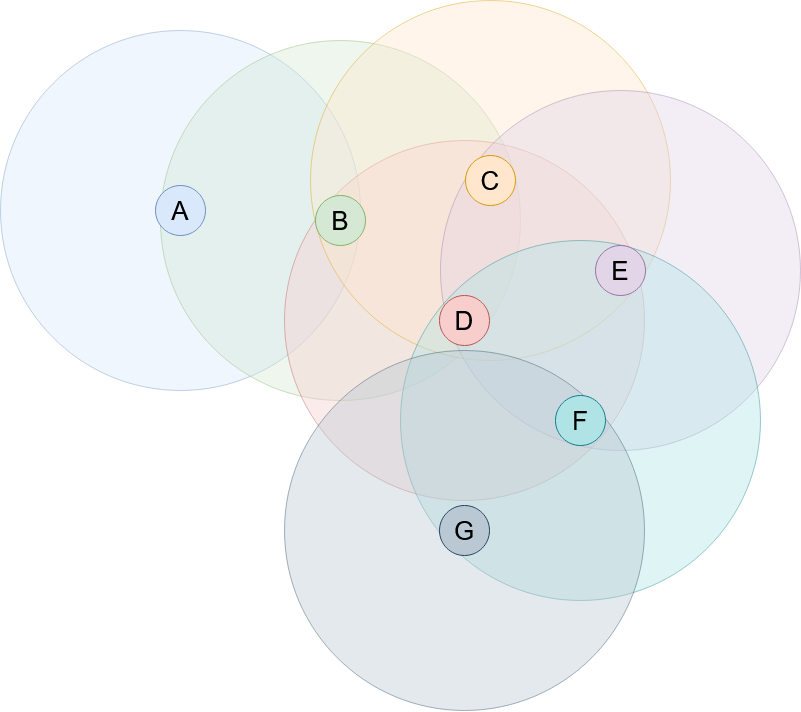
\includegraphics[scale=0.19]{img/wireless_graph_1.png} }}%
    \qquad
    \subfloat[\centering Equivalent graph representation]{{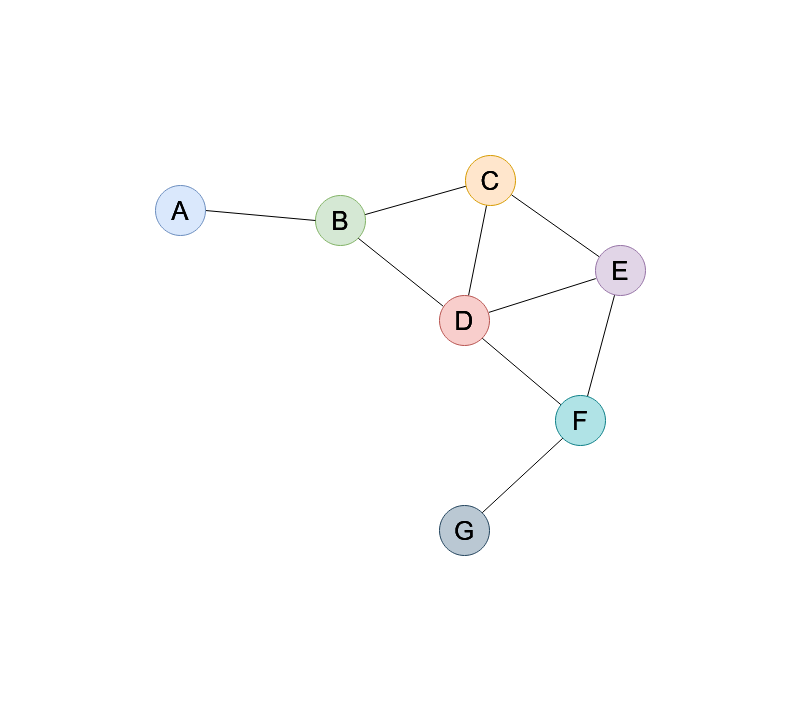
\includegraphics[scale=0.19]{img/wireless_graph_2.png} }}%
    \caption{}%
    \label{fig:graph1}%
\end{figure}

In Figure \ref{fig:graph1} (a) devices A, C and D are within device B transmission radius. In the equivalent graph, there will be edges that connect B to A, B to C and B to D. The same goes for all the other vertices.\\
In general, the existence of an edge from vertex $i$ to vertex $j$ means that nodes $i$ and $j$ are within reach of each other. Two vertices connected by an edge are said to be \textit{adjacent}. The set of a vertex $v$ together with all its adjacent nodes forms a subgraph called the \textit{neighbourhood of v}.\\
During the broadcast, a node can only receive from and transmit to its neighbourhood.\\
\hfill \break
Once a node has transmitted the message and has gone into \texttt{sleeping} state, it disappears, along with all the edges connected to it. Therefore, the set of vertices V changes with time. This is what in literature is called a \textit{dynamic graph} or, more specifically, a \textit{node-dynamic graph.}

%Should this paragraph be moved to another chapter/section ?
Modelling the system with graphs also allows for the easy computation of a lower bound for the broadcast time \texttt{T}, which can be useful for the validation of the simulator.\\
Given a graph $G(V, E)$ that represents the users in the floorplan, let $v^{*}$ be the starter of the broadcast, i.e. the first node with the message.\\
In a best case scenario, the system evolves with no collisions at all and the message moves along the paths of the graph, reaching all nodes.\\
%TODO add citation to bibliography: [ F. Harary, Graph Theory, Addison-Wesley, 1969, p.199. ]
Let $d(u, v)$ be the \textit{distance} between two vertices $u$ and $v$, i.e. the length of a shortest directed path from u to v consisting of arcs, provided at least one such path exists.\\
Then, the lower bound for the broadcast time is given by the greatest distance between $v^{*}$ and any other vertex. This quantity, in graph theory, is called \textit{eccentricity} of the vertex $v^{*}$. More formally, the eccentricity of $v^{*}$ is defined as follows:

\begin{equation}
\epsilon(v^{*}) = \max_{v{\in}V} d(v^{*}, v)
\end{equation}



\section{Simplified models}

\subsection{Single queue configuration}

Let us consider a configuration where devices arranged in a line, as shown in Fig. \ref{fig:single_queue}. Each device only has two neighbours, except for the outer ones that only have one. Let assume A to be the broadcast starter. A is in \texttt{transmitting} state while all the other nodes are initially in \texttt{listening} state. 
\hfill \break
\hfill \break

\begin{figure}[H]%
    \centering
	{{
\includegraphics[scale=0.6]{img/single_queue.png} }}%
    \caption{}%
    \label{fig:single_queue}%
\end{figure}

It is clear that, with this configuration, each listening node has a maximum of one active node in its neighbourhood and thus cannot possibly receive the message from two different sources at the same time.
This guarantees the absence of collisions.

In such a scenario, $100\%$ asymptotic coverage is ensured:
during each slot, the active node extracts a Bernoulli RV with success probability $p$. The probability of the active node not transmitting for k consecutive slots is a geometric distribution:

\begin{equation}
	P(X = k) = (1\text{-}p)^{k}
	\label{geometric_distribution}
\end{equation}

The successful transmission of the message from an active node to its neighbour is thus guaranteed since $\lim_{k \to \infty} (1\text{-}p)^{k} = 0$

%TODO not really sure about this result when the starter node is not the first or the last. What if the starter node is in the middle of the queue?
As for the total broadcast time \texttt{T}, on average it is equal to the mean value of the Bernoulli RV, \textit{p}, times the number of hops needed to reach the last node.
%times the eccentricity of the starter, maybe? Not really sure about that, I have to look into it a bit more in detail

\subsection{Star configuration}
Another useful simple configuration worth analysing is a star-shaped configuration. In this setup, there is a central node A connected to N-1 nodes, all of which are non-adjacent. Let us suppose A to be the broadcast starter.

\begin{figure}[H]%
    \centering
	{{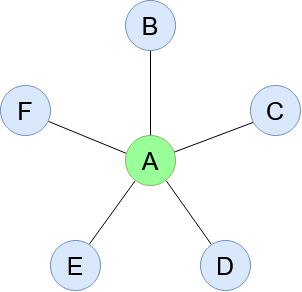
\includegraphics[scale=0.5]{img/star_graph.png} }}%
    \caption{}%
    \label{fig:star_graph}%
\end{figure}

The absence of collisions is ensured in this scenario as well, for the same reason as the previous example.\\
At each slot, A keeps extracting a Bernonulli RV. When the extraction is successful, A broadcasts the message to all its neighbour and total coverage is reached. Hence, 100\% asymptotic coverage is ensured in this case too, as the probability of A not transmitting for k consecutive slots is Eq. \ref{geometric_distribution} and goes to 0 as k goes to infinity.\\
In this case, the average total broadcast time $E[\texttt{T}]$ is simply equal to the mean value of the Bernoulli RV \textit{p}.

If the broadcast starter was one of the ``rays" of the star, instead of the center, there would not be much difference: absence of collisions and total coverage would be ensured as well.\\
As for \texttt{T}, its expected value would just be $2p$, since the starter would have to transmit the message to the center of the star and then the resulting setup is reduced to the previous one.